\section{Work Efficiency} \label{sec:work}

    In this section, we introduce \textit{work efficiency}, a novel performance metric for comparing the quality of different optimized
    versions of a program, even when we evaluate them with a different input each time. Similarly to existing one-shot performance metrics,
    work efficiency is simply the amount of \textit{work done per unit of time}: 
    \[
        \textrm{Work Efficiency} = \frac{\Delta W}{\Delta t}
    \]
    where $\Delta W$ is the amount of work performed during a period of time $\Delta t$.

    With similar metrics, what exactly is work depends on the application and is defined by the developer: SQL queries executed,
    transactions completed, bytes processed, etc. In our case, we need a similar but application-agnostic metric which correlates with what
    the developer considers useful work and is simple enough to be calculated online.

    Section~\ref{subsec:workmetric} describes this new work metric and the design choices we made, Section~\ref{subsec:prof} details how
    we measure work, and Section~\ref{subsec:relaxed} explores ways to measure it with reduced interference on %without interfering with
    the normal operation of the program.

    \subsection{Work Metric} \label{subsec:workmetric}

    To build a reasonable work metric, our approach starts by assuming that each executed instruction\footnote{In this paper, we consider instructions at the level of the Intermediate Representation (IR) of the LLVM compiler.} contributes a certain amount towards
    the total useful work. To keep the measurement simple and minimize the online overhead, we assume that the contribution depends only on
    the type of instruction. Additionally, we would expect two program versions processing the same data in the same way to do the same
    work. If measured using the actual instructions executed for the two versions, we would get a different amount of work. Instead, we
    increase the total work based on the instructions that would be executed with the unoptimized code, regardless of the version we use.
    The unoptimized version is convenient as a common baseline, since we start with it anyway and it is as close as possible to the
    programmer's intention.

    We selected the work contribution of each instruction type so that total work becomes an estimator of the runtime of the unoptimized
    program.
    %Our choice to associate work with unoptimized runtime is largely arbitrary but instinctively reasonable.
    Our choice to associate work with unoptimized runtime is largely for practical reasons but it is also instinctively reasonable.
    Unoptimized time is
    close to how the programmer understands the effort put by the computer. Using it as the work metric makes work efficiency (work per unit
    of time) an estimator of the speedup of the optimized version over the unoptimized version. While other ways of setting the instruction
    contributions might be better, our results in Section~\ref{sec:results} show that this simple definition of work produces good results.
    Using the experimental setup described in Section~\ref{sec:setup}, we run the unoptimized versions of the 10 benchmarks listed in
    Table~\ref{tab:kdatasets:training} with all 1,000 available inputs. For each run, we recorded execution time and dynamic counters for all instruction types\footnote{
    Dynamic instruction counts were obtained by using the classic block-frequency profiling.}.
    Similarly to prior work~\cite{giusto01,powell09,brandolese11}, we then applied linear regression to find the contribution of each
    instruction type that minimizes the error between measured runtime and work.
    %\footnote{The resulting regression model uses \FIXME{70}
    %different instruction types which make it too long to present here.}

%%    \begin{figure}[t]
%%        \centering
%%        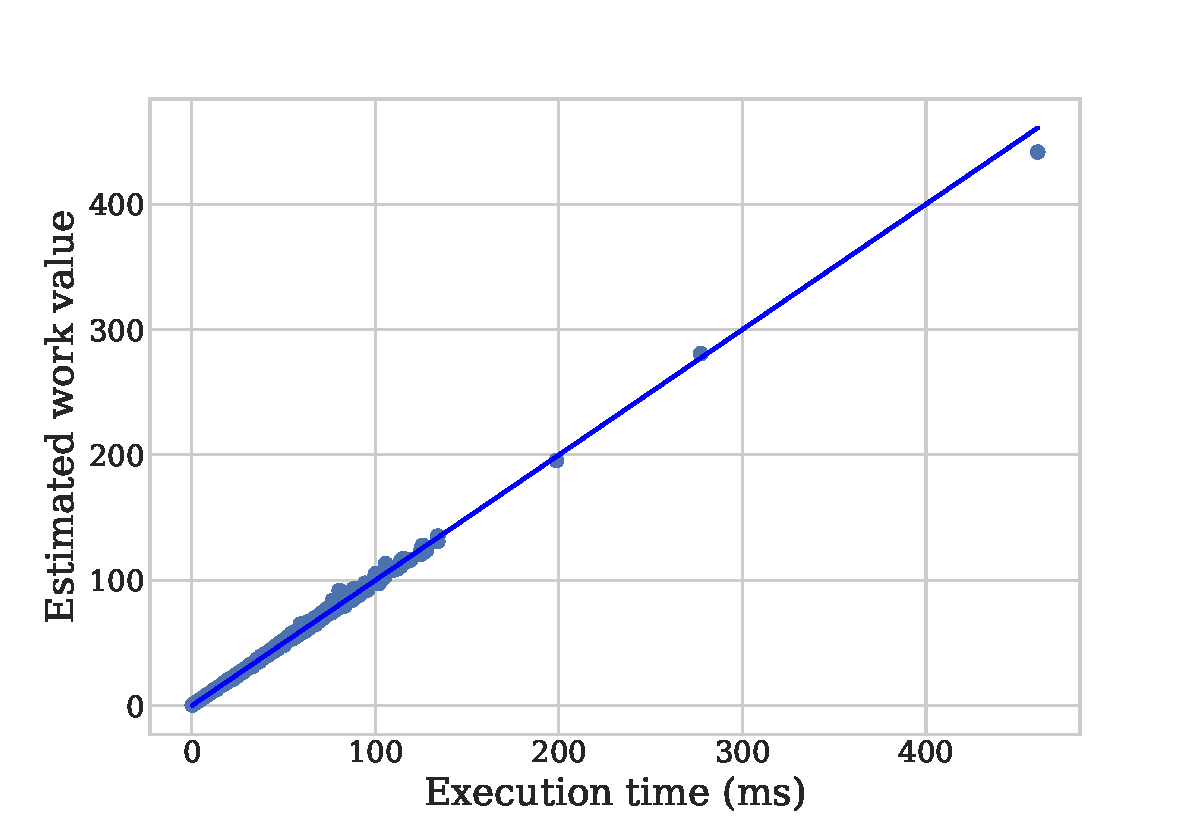
\includegraphics[width=0.5\textwidth]{figs/work-correlation-with-O0_susan_c.pdf}
%%        \caption{
%%            Relationship between work metric ($\Delta W$) and the execution time of the unoptimized version of the \texttt{susan\_c}
%%            benchmark over the 1,000 inputs. Each point represents the execution of a single input. They have a correlation coefficient of
%%            $0.99$.
%%        }
%%        \label{fig:work-vs-O0time}
%%    \end{figure}
    
    Figure~\ref{fig:motivation-speedups} shows the correlation coefficient between the work metric ($\Delta W$) and the runtime of the
    unoptimized version for 14 benchmarks that were not used for training the linear model. The work metric correlates very strongly with
    runtime for almost all the benchmarks, the correlation coefficient being typically higher than $0.98$. The exception is the benchmarks
    based on \texttt{tiff}. The coefficient for them ranges from $0.47$ to $0.96$. Despite that, in most cases work is an excellent proxy
    for unoptimized runtime. For the rest, our Section~\ref{sec:results} evaluation shows that our work metric is still useful for quantifying
    performance. 


\begin{figure*}[t]
    \centering
    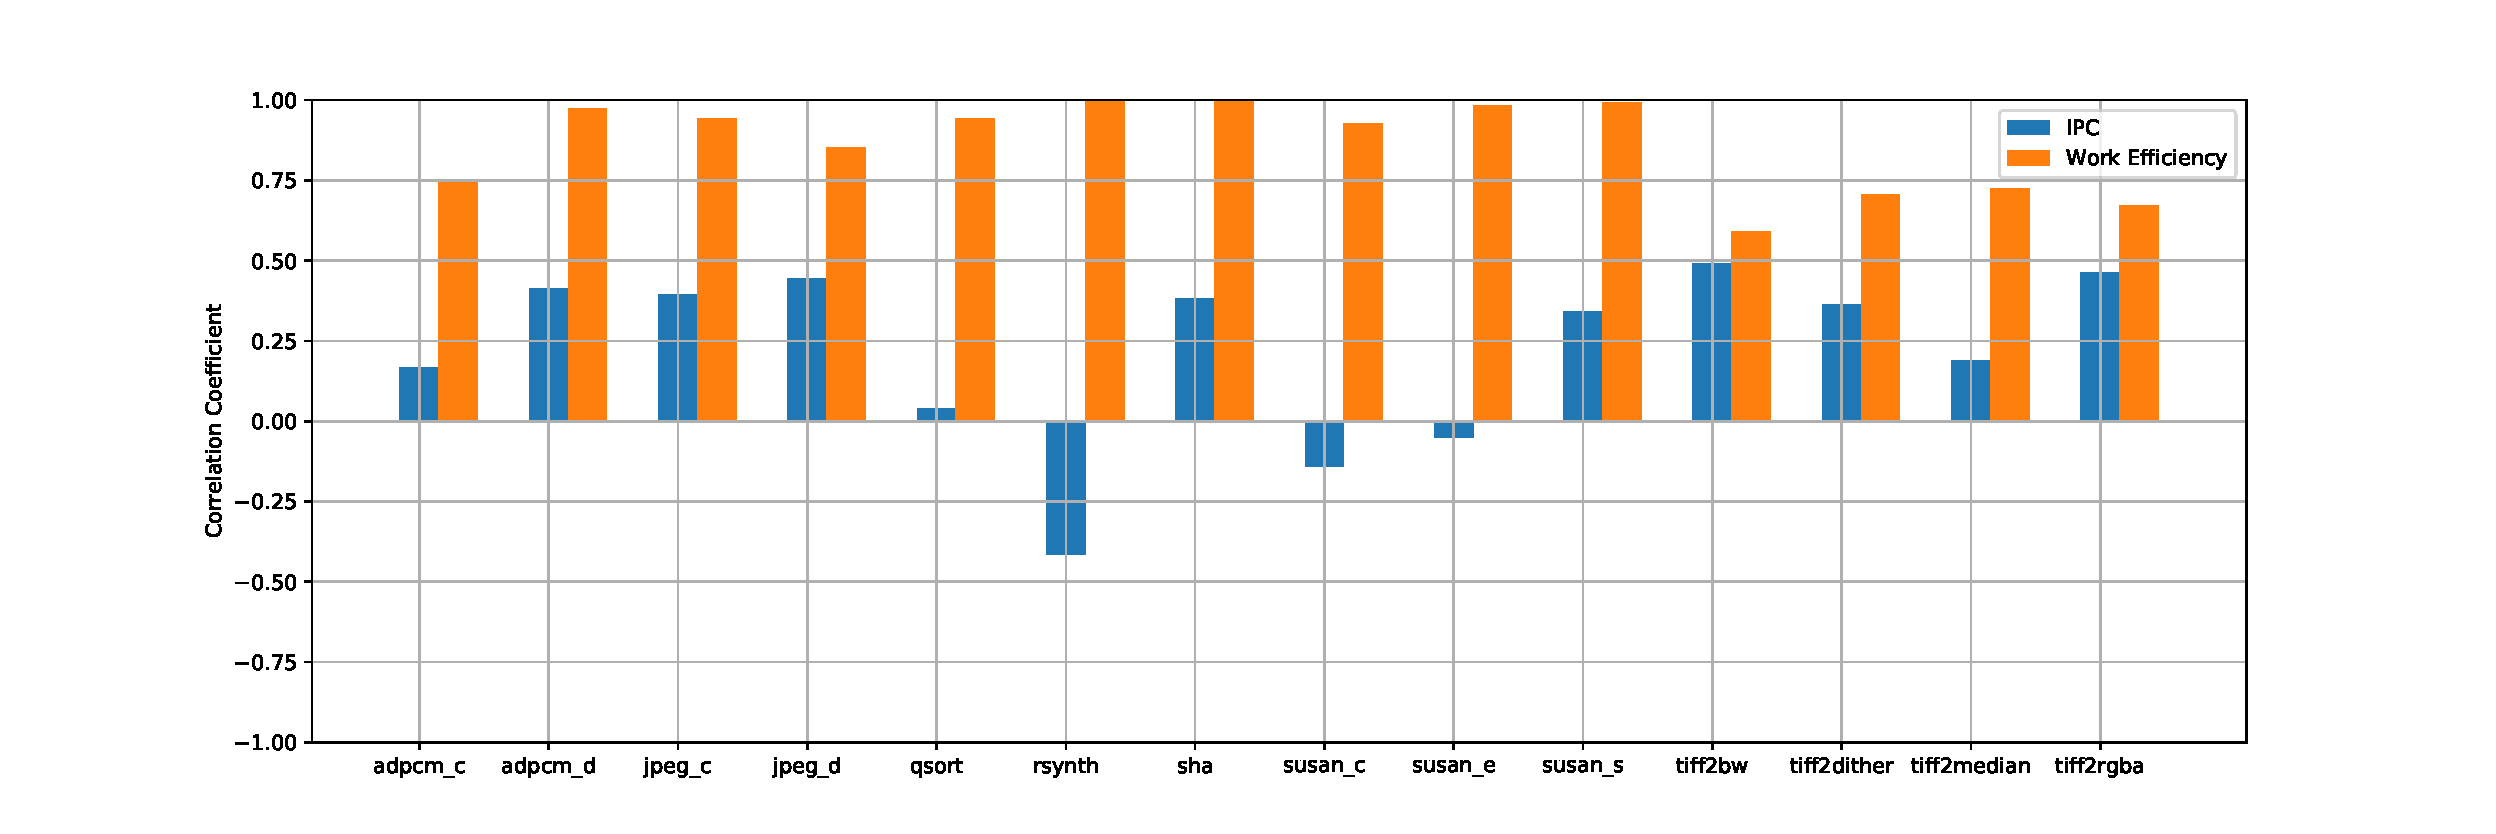
\includegraphics[width=\textwidth]{figs/corr_coeff.pdf}
    \caption{Correlation coefficients between the work metric ($\Delta W$) and the execution time of the unoptimized version for each benchmark.}
    \label{fig:motivation-speedups}
\end{figure*}


    \subsection{Work Profiling}\label{subsec:prof}

    Total work is just the sum of the cost of all instructions that would be executed in the unoptimized binary. A na\"{\i}ve but
    straightforward way to measure work online is to instrument the unoptimized code with a global work counter and instructions for
    incrementing this counter after each instruction of the original code. Since the work contribution of each instruction depends only on
    its type, it can be determined at compile time. Taking this one step further, we can calculate work contributions at the basic block
    level and insert only a single increment instruction in each block. Although easy to implement, the na\"{\i}ve approach introduces a
    significant overhead.

    Previous work on basic block profiling has proposed ways for instrumenting the code with as little overhead as possible without losing
    any profiling information~\cite{knuth73,ball94}. The underlying idea is that we can still calculate precisely the execution counts of
    all basic blocks if we choose a spanning tree of the function Control Flow Graph (CFG) and only instrument the edges of the CFG
    \textit{not} in the tree~\cite{nahapetian73,forman81}. To make the instrumentation probe placement optimal, we choose the maximum
    spanning tree, with the edge weights representing edge frequency estimates. This maximises the number of high frequency edges that will
    not be instrumented, minimizing the instrumentation cost~\cite{forman81,ball94}. 
    
    \begin{figure}[t]
    \centering {
      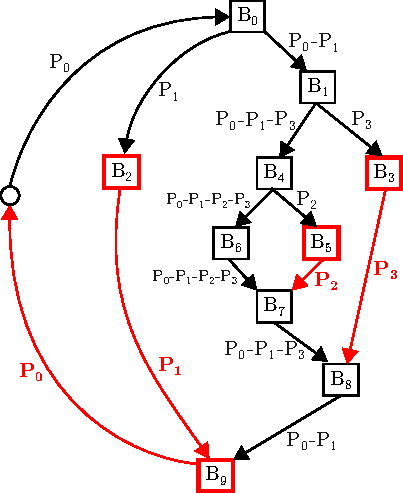
\includegraphics[scale=0.8]{figs/cfg-example.pdf}\\\vspace{1ex}
      \resizebox{0.45\textwidth}{!}{
      %\scalebox{0.8}{
         \begin{minipage}{0.5\textwidth}
         Instrumented value for each probe $P_i$:
         \begin{align*}
         \omega(P_0) &= w(B_0) + w(B_1) + w(B_4) + w(B_6) + w(B_7) + w(B_8) + w(B_9)\\
         \omega(P_1) &= w(B_2) - w(B_1) - w(B_4) - w(B_6) - w(B_7) - w(B_8)\\
         \omega(P_2) &= w(B_5) - w(B_6)\\
         \omega(P_3) &= w(B_3) - w(B_4) - w(B_6) - w(B_7)
         \end{align*}
         \end{minipage}
      }
    }
      \caption{Example of a CFG with its maximum spanning tree in black. Basic blocks and edges highlighted in red are instrumented.
        Instrumenting them is enough for calculating the total work performed by the whole CFG.}
      \label{fig:cfg-example}
    \end{figure}

    With na\"ive instrumentation each basic block records only its own amount of work. With optimal probe placement, reaching a probe
    implies not only executing the containing block but also executing or not executing other uninstrumented blocks, so work counter
    increments have to reflect this. Figure~\ref{fig:cfg-example} shows an example CFG, where the instrumented blocks are marked with red.
    In this example, reaching probe $P_2$ implies not only executing block $B_5$ but also not executing $B_6$.
    
    To compute the amount of work associated with each instrumentation probe, we first need to determine how reaching a probe relates with
    executing or not a basic block. Starting from instrumented edges, we use Kirchhoff's first law~\cite{knuth73,ball94} and a post-order
    traversal of the spanning tree to build symbolic expressions of edge frequencies as linear functions of probe counts, as seen in
    Figure~\ref{fig:cfg-example}. This part is similar to how edge and block frequencies are calculated in prior work for basic block
    profiling, with a few key differences:
    (i)   work profiling does not have to store the execution count of each basic block, only the total work which makes it cheaper to profile;
    (ii)  it does not require a post-processing of the recorded profiling for populating the edge flows;
    (iii) the propagation of the edge flows happens in a symbolic fashion during the instrumentation of the code, as depicted in Figure~\ref{fig:cfg-example}.
    This symbolic edge flows are used to derive the frequency expression of the basic blocks, which is then used to derive the amount of work
    recorded by each probe.
    
    %Simply put, the sum of the frequencies of the edges entering a block and the sum of the frequencies
    %exiting the same block must match. Starting from the leaf nodes of the spanning tree, where by definition all edges except one should
    %be instrumented, and working upwards, we should be able to calculate the frequencies of all nodes and edges as a function of the probe
    %of the probe counts.
    
    If a block's frequency expression contains a positive term for a probe, this means that the block is executed when we reach the probe,
    so the block's cost should be added at that probe. Conversely, if the expression contains a negative term for a probe, then the block
    is executed when we do not reach the probe, so the block's cost should be subtracted. In our example CFG, the symbolic expression for
    the basic block $B_8$ is $P_0 - P_1$, so the amount of work of $B_8$, denoted by $w(B_8)$, is incremented in probe $P_0$ and
    decremented in $P_1$.


    \subsection{Relaxed Instrumentation}\label{subsec:relaxed}

    Optimal instrumentation significantly reduces the profiling overhead when compared to na\"ive instrumentation, from an average overhead
    of 79\% to 13\%. Still, 13\% slowdown might be more than what the user is ready to tolerate, while for isolated case the overhead might
    be as high as 60\%. We need to reduce overhead further to make the work metric practical. 
    
    We propose two novel relaxation strategies that offer a trade-off between accuracy and overhead. Our insight was that, unlike basic
    block profiling, not all probes are of equal importance. The work associated with some is insignificant compared to the total work
    done by the program, so ignoring them will have little negative impact on the accuracy of measuring work. By removing such probes,
    especially if they are frequently executed, we can reduce the instrumentation overhead dramatically. These two strategies are
    particular to work profiling and reduce the overhead much more than what previous research in basic block profiling has achieved. 

    To select which probes to remove we consider the probes in a control flow region. The runtime benefit of removing a probe is
    proportional to the frequency of the block the probe is in, while the error introduced is proportional to both the work contribution of
    the probe and its frequency. We solve the 0-1 Knapsack optimization problem, removing probes to maximize the total savings while
    keeping the accumulated error below a threshold:
    \begin{gather*}
        \textrm{max.}\quad\sum_{i=0}^{k} f(P_i)x_i,\quad
        \textrm{s.t.}\quad\sum_{i=0}^{k} \varepsilon(P_i)x_i \leq M \\
        x_i\in\{0,1\}, i\in\{0,\ldots,k\}
    \end{gather*}
    where the set of probes in the region being considered is $\{P_0, P_1, \ldots, P_k\}$, $f(P_i)$ is the execution frequency of probe
    $P_i$ and $x_i$ denotes the probes selected for removal, $\varepsilon(P_i)$ is the error for removing $P_i$ and $M$ is the maximum
    error threshold.

    For our experiments, we implemented two solvers for the 0-1 Knapsack problems: an optimal but potentially slow brute-force solver and a
    greedy heuristic based on sorting the items~\cite{dantzig57}. We use the brute-force solver with a small number of probes, less than
    20, and the greedy heuristic otherwise.

    We have two relaxation strategies which differ in the control flow regions they tackle and how they calculate the error terms. The
    first is a more conservative approach that calculates induced error from removing a probe by considering the worst case of any
    execution path through the program. The second is a more aggressive approach that computes induced error based on the relative change
    of the work measurement that removing a probe would make to the total amount work for the whole program. We discuss each one of them
    in detail.

    \subsubsection{\WCRelaxTitle Relaxation}

    In order to offer hard guarantees for the error upper bound, this conservative approach first decomposes the CFGs of the program into
    subgraphs where the maximum possible work contributed by each probe, as well as the minimum possible amount of total work for the whole
    subgraph, can be calculated. Then, it removes probes within each subgraph while keeping the maximum possible error rate for that
    subgraph bounded by the threshold. With the error rate of each subgraph below the threshold, it is guaranteed that the dynamic error of
    the work metric for the whole program will always be bounded by the threshold.

    \begin{figure}[t]
      \centering
      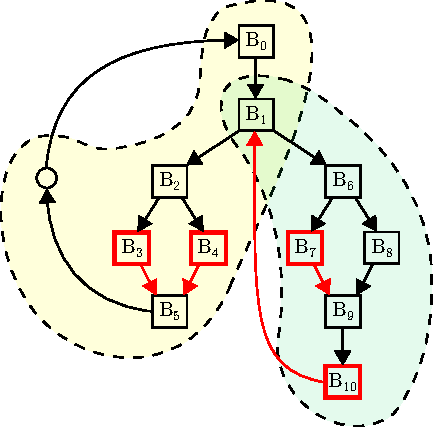
\includegraphics[scale=0.8]{figs/cfg-relax-example.pdf}
      \caption{Example of a CFG containing a loop and its decomposition into DAGs.
               The DAGs are the subgraphs within the dashed boundaries.}
      \vspace{-4mm}
      \label{fig:cfg-relax-example}
    \end{figure}

    The \WCRelaxLower relaxation starts by extracting directed acyclical graphs (DAGs) from the CFG. The algorithm extracts subgraphs that
    represent loops or the outer most region of the function. The subgraphs are transformed into DAGs by ignoring the backedge and moving
    inner loops to their own subgraphs. An example of this is shown in Figure~\ref{fig:cfg-relax-example}, where the CFG is partitioned
    into two DAGs.

    Since there are no loops in the DAG, we can determine $m$, the minimum amount of work that can be done in a single execution of the
    DAG. For the same reason, the maximum amount of work that a probe can contribute is when it is reached once. Given this, the worst case
    relative error caused by removing a probe $P_i$ is $\varepsilon(P_i) = \frac{\omega(P_i)}{m}$. By repeating the same process for
    all DAGs of the CFG, we guarantee that the final error introduced by relaxation will always be below the chosen threshold.

    \subsubsection{\WPRelaxTitle Relaxation}

    The \WCRelaxLower relaxation error guarantees are hard but also too conservative. It assumes that each loop will always execute the
    path with the minimum amount of work possible, which might be orders of magnitude less than the work actually performed. When this is
    the case, we end up with a relative error much lower than intended and a profiling overhead unnecessarily high. Our second, more
    aggressive, strategy avoids this problem, by estimating the error and overhead contributions of each probe in relation to the whole
    program. 

    The \WPRelaxLower relaxation does this by using block-frequency profiling from previous executions. With this information, we are able
    to estimate the probe frequencies and the relative error of removing a given probe in terms of total program work. We select a subset
    of all the probes to be removed, while keeping the total relative error (over total program work) below the threshold.
    
    Contrary to the per DAG approach, the error introduced by \WPRelaxLower relaxation is not guaranteed to be bounded by the threshold
    $M$. Still, we expect it to remain close to the threshold as long as the program's behavior does not deviate significantly from the
    behavior captured in the profile we used.
